\documentclass[11pt,spanish,a4paper]{article}
% Versión 1.er cuat 2021 Víctor Bettachini < bettachini@df.uba.ar >

% Versión 1.er cuat 2021 Víctor Bettachini < bettachini@df.uba.ar >

\usepackage[T1]{fontenc}
\usepackage[utf8]{inputenc}

\usepackage[spanish, es-tabla]{babel}
\def\spanishoptions{argentina} % Was macht dass?
% \usepackage{babelbib}
% \selectbiblanguage{spanish}
% \addto\shorthandsspanish{\spanishdeactivate{~<>}}

\usepackage{graphicx}
\graphicspath{{./figuras/}{../LaTeX/}}
% \usepackage{float}

\usepackage[arrowdel]{physics}
\newcommand{\pvec}[1]{\vec{#1}\mkern2mu\vphantom{#1}}
% \usepackage{units}
\usepackage[separate-uncertainty=true, multi-part-units=single, locale=FR]{siunitx}
\usepackage{isotope} % $\isotope[A][Z]{X}\to\isotope[A-4][Z-2]{Y}+\isotope[4][2]{\alpha}

\usepackage{tasks}
\usepackage[inline]{enumitem}
% \usepackage{enumerate}

\usepackage{hyperref}

% \usepackage{amsmath}
% \usepackage{amstext}
\usepackage{amssymb}

\usepackage{tikz}
\usepackage{tikz-dimline}
\usetikzlibrary{calc}
% \usetikzlibrary{math}
\usetikzlibrary{arrows.meta}
\usetikzlibrary{snakes}
\usetikzlibrary{decorations}
\usetikzlibrary{decorations.pathmorphing}
\usetikzlibrary{patterns}

% \usepackage[hmargin=1cm, vmargin=1cm, includeheadfoot]{geometry}
\usepackage[hmargin=1cm,vmargin=3cm, top= 0.75cm,nohead]{geometry}
% \voffset-3.5cm
% \hoffset-3cm
% \setlength{\textwidth}{17.5cm}
% \setlength{\textheight}{27cm}

\usepackage{lastpage}
\usepackage{fancyhdr}
\pagestyle{fancyplain}
\fancyhf{}
% \fancyhead{}
\setlength\headheight{28.7pt} 
\fancyhead[LE, LO]{\textbf{Física 2} (Físicos) }
% \lhead{\textbf{Física 2} (Físicos) }
\fancyhead[RE, RO]{\href{https://df.uba.ar/es/}{$\vcenter{\hbox{\includegraphics[height=1cm]{sin_texto.pdf}}}$}}
% \rhead{$\vcenter{\hbox{\includegraphics[height=1cm]{sin_texto.jpg}}}$}
% \rhead{\includegraphics[height=1cm]{sin_texto.jpg}}
% \rhead{\textcopyright {\tt DF, FCEyN, UBA}}
\fancyfoot{\href{https://creativecommons.org/licenses/by-sa/4.0/deed.es/}{$\vcenter{\hbox{\includegraphics[height=0.4cm]{cc-by-sa.pdf}}}$} \href{https://df.uba.ar/es/}{DF, FCEyN, UBA}}
% \fancyfoot{$\vcenter{\hbox{\includegraphics[height=0.4cm]{cc-by-sa.pdf}}}$ DF, FCEyN, UBA}
% \fancyfoot{{\tiny \textcopyright DF, FCEyN, UBA}}
\fancyfoot[C]{ {\tiny Actualizado al \today} }
\fancyfoot[RO, LE]{Pág. \thepage/\pageref{LastPage}}
\renewcommand{\headrulewidth}{0pt}
\renewcommand{\footrulewidth}{0pt}


\begin{document}
\begin{center}
\textbf{Física 2} (Físicos) \hfill \textcopyright {\tt DF, FCEyN, UBA}\\
	\textsc{\LARGE Sistemas periódicos}
\end{center}

Los ejercicios con (*) son opcionales.

\begin{enumerate}



\section*{Modos normales en sistemas periódicos}


\item
\begin{minipage}[t][1cm]{0.45\textwidth}
Para el sistema de $N$ masas de la figura. 
\end{minipage}
\begin{minipage}[c][1.5cm][t]{0.5\textwidth}
  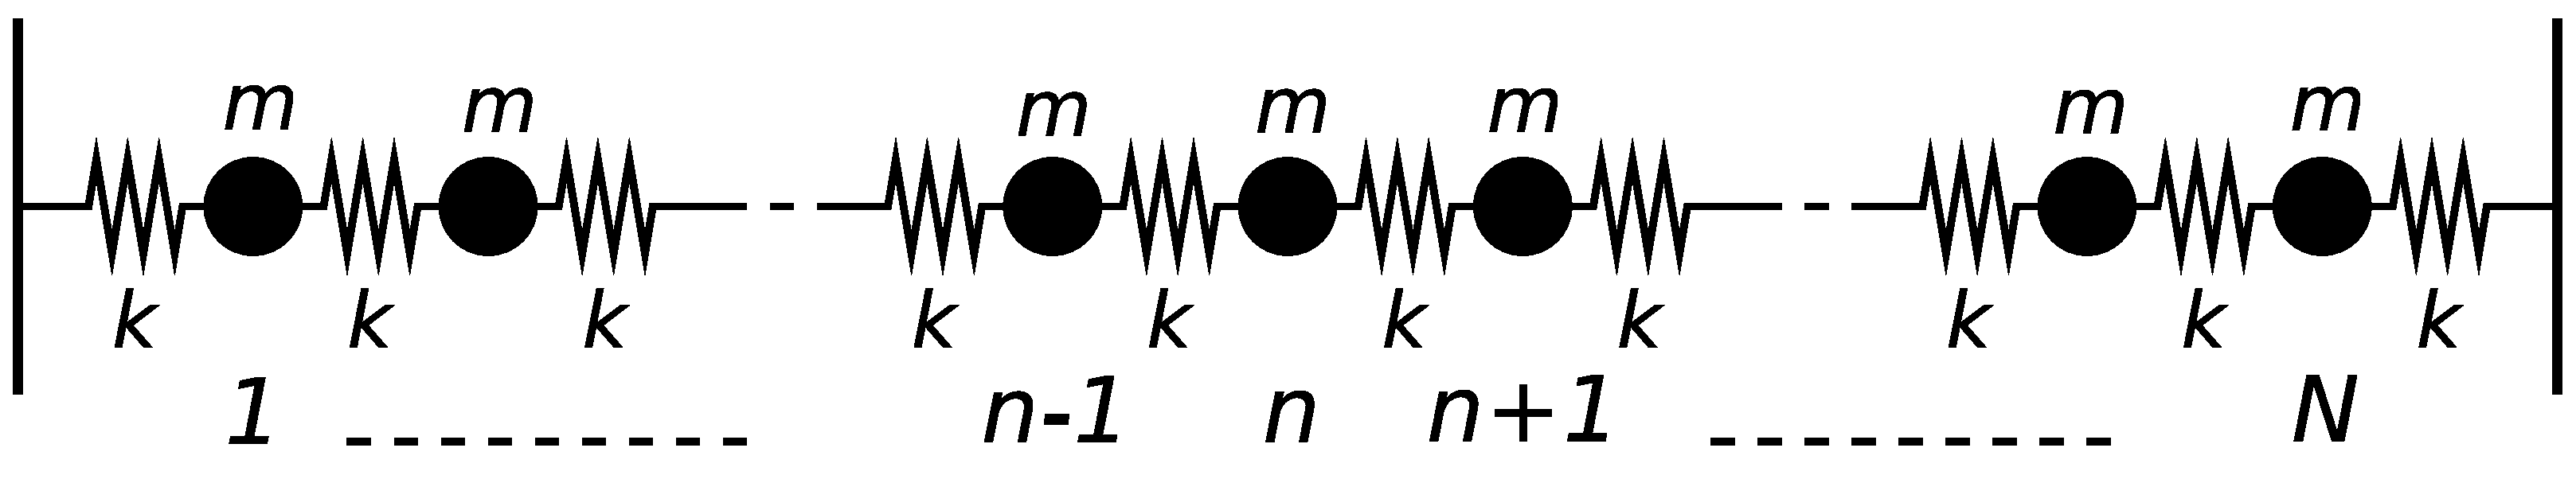
\includegraphics[width=\textwidth]{ej1-11}
\end{minipage}
\begin{enumerate}
	\item Escriba la ecuación de movimiento transversal para la partícula enésima usando la aproximación de ángulos pequeños.
	\item Proponga una solución de la forma:
	\[
		\Psi_{n}^{(p)}(t)=A^{(p)}\cos\left(nk^{(p)}a+\alpha^{(p)}\right)\cos\left(\omega^{(p)}t+\phi^{(p)}\right)
	\]
	Halle la relación de dispersión y grafíquela.
	¿Depende esta relación de las condiciones de contorno?
	¿Cuánto vale la frecuencia más baja?
	¿Qué representa dicho modo? 
	\item Obtenga las frecuencias correspondientes a los modos normales cuando ambos extremos están libres (atención: ¿cómo sería un ``extremo libre'' en esta configuración?) y escriba la solución general para la masa enésima. 
	\item Ídem. anterior, pero con el extremo izquierdo libre y el derecho fijo a la pared. 
	\item Particularice los resultados de los dos ítems anteriores para el caso en que $N=3$.
\end{enumerate}



\item
\begin{minipage}[t][2cm]{0.6\textwidth}
 Considere el sistema de péndulos acoplados de la figura. 
\end{minipage}
\begin{minipage}[c][2cm][t]{0.35\textwidth}
  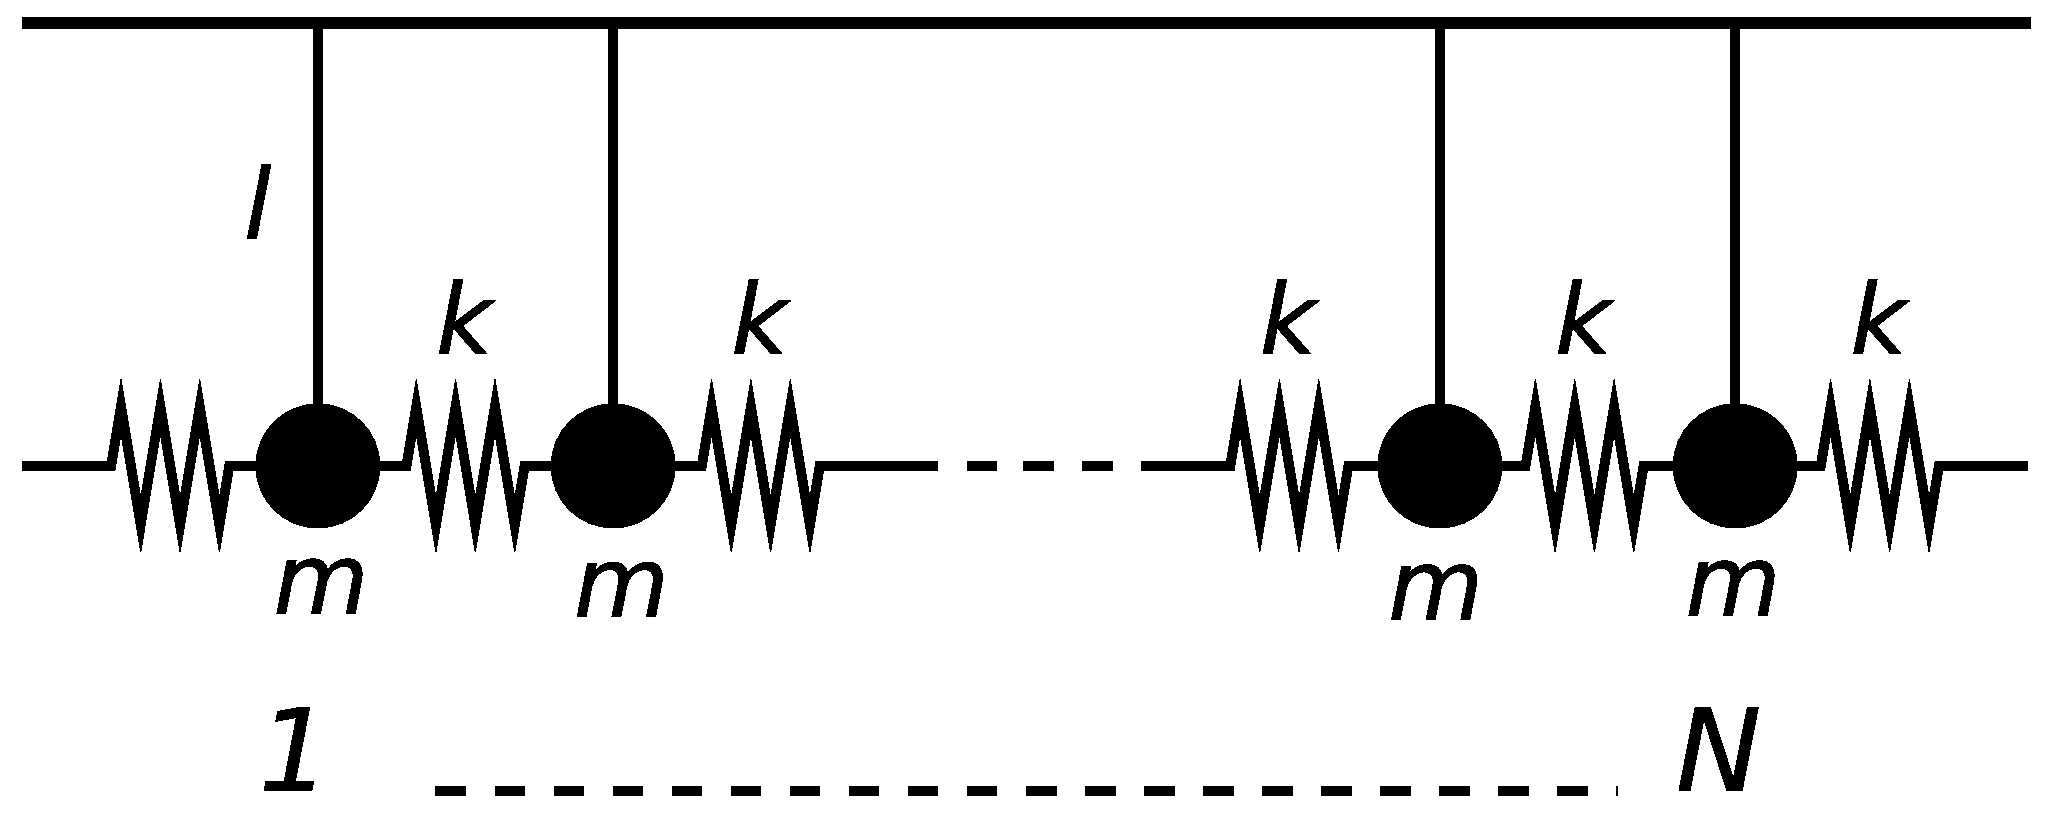
\includegraphics[width=\textwidth]{ej1-12}
\end{minipage}
\begin{enumerate}
	\item Escriba la ecuación de movimiento. Proponga una solución semejante a la del problema anterior y halle la relación de dispersión. Compárela con la obtenida en el problema anterior.
	¿Cuánto vale la frecuencia más baja?
	¿Qué representa dicho modo? 
	\item Obtenga las frecuencias correspondientes a los modos normales cuando los resortes de los extremos están fijos y dé las condiciones iniciales para excitar el primer armónico. 
	\item Ídem anterior, pero para el caso en que uno de los resortes de los extremos está libre. 
\end{enumerate}


\subsection*{Oscilaciones forzadas de sistemas con N grados de libertad}

\item Considere el sistema de dos péndulos acoplados, tal que uno de ellos es impulsado por una fuerza $F= F_0 \cos(\Omega t)$.
Desprecie el amortiguamiento.
Muestre que:
\[
\Psi_a \approx \frac{F_0}{2M} \cos(\Omega t) \left[\frac{1}{\omega_1^2- \Omega^2} + \frac{1}{\omega_2^2- \Omega^2}\right];
\]
\[
\Psi_b \approx \frac{F_0}{2M} \cos(\Omega t) \left[\frac{1}{\omega_1^2- \Omega^2} - \frac{1}{\omega_2^2- \Omega^2}\right];
\]
\[
\frac{\Psi_b}{\Psi_a} \approx \frac{\omega_2^2- \omega_1^2}{\omega_2^2+ \omega_1^2- 2 \Omega^2};
\]
donde $\omega_{1}$ es la menor de las frecuencias modales, $\omega_2$ es la mayor y $\Omega$ es la frecuencia de excitación.



\item
\begin{minipage}[t][3.5cm]{0.7\textwidth}
Considere el sistema de 3 péndulos acoplados que se muestra en la figura.
\begin{enumerate}
	\item Escriba la ecuación de movimiento para cada masa y encuentre las frecuencias
	propias y los modos normales del sistema. 
	\item Suponga que en el extremo libre se aplica una fuerza $F= F_0 \cos(\omega t)$.
	Escriba la ecuación de movimiento para cada masa y encuentre la solución estacionaria para cada modo.
	¿Cuáles son las frecuencias de resonancia?
\end{enumerate}
\end{minipage}
\begin{minipage}[c][0cm][t]{0.25\textwidth}
  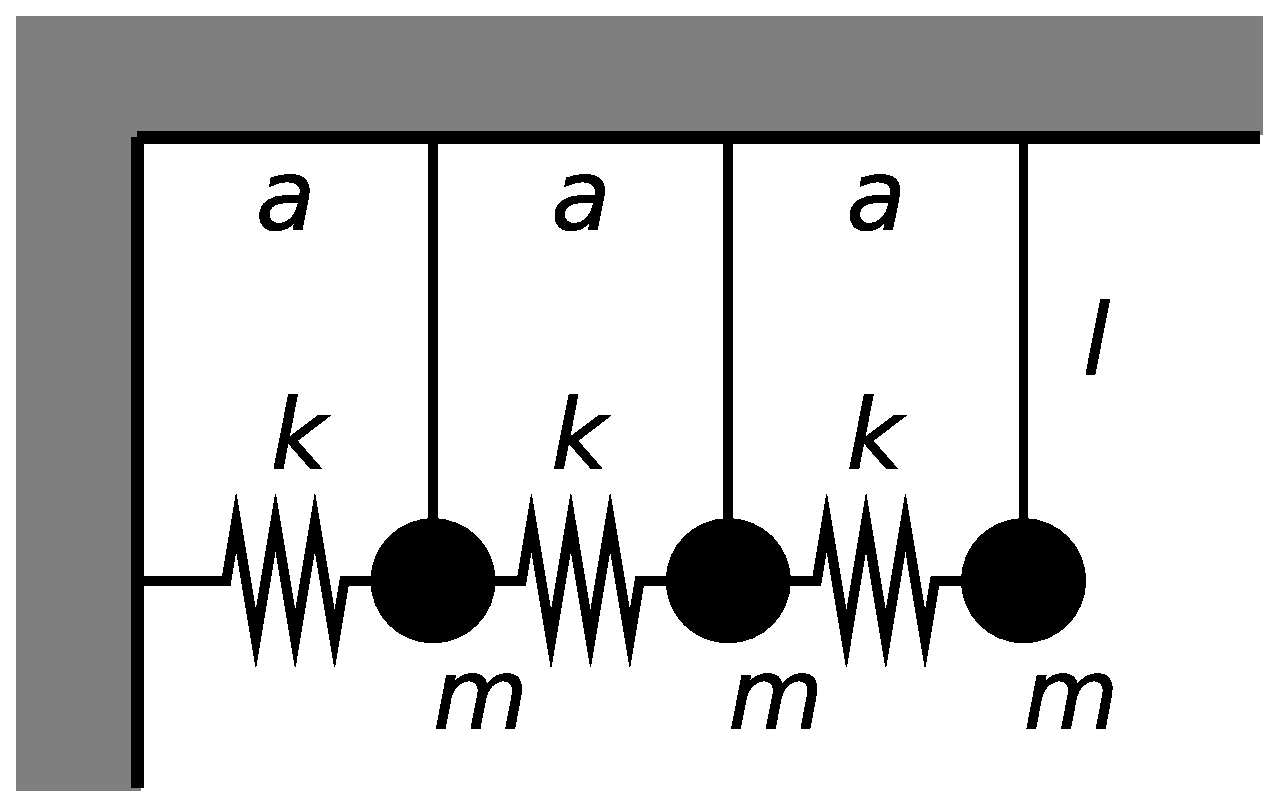
\includegraphics[width=\textwidth]{ej1-14}
\end{minipage}



\subsection*{Oscilaciones forzadas de sistemas periódicos}


\item
\begin{minipage}[t][3.5cm]{0.6\textwidth}
En este arreglo lineal de péndulos acoplados excitados tiene extremos en $z= 0$ y en $z= L$.
Se aplica una fuerza externa en función del tiempo a la primera masa ($z=0$), de forma tal que se conoce su amplitud $\Psi(0,t)= A_0 \cos(\Omega t)$.
Halle el movimiento estacionario del sistema y discuta las hipótesis que hace.
Compare con el caso de extremo derecho fijo a una pared (o sea: agregando un resorte a la derecha de la última masa y uniéndolo a la pared). 
\end{minipage}
\begin{minipage}[c][0cm][t]{0.35\textwidth}
  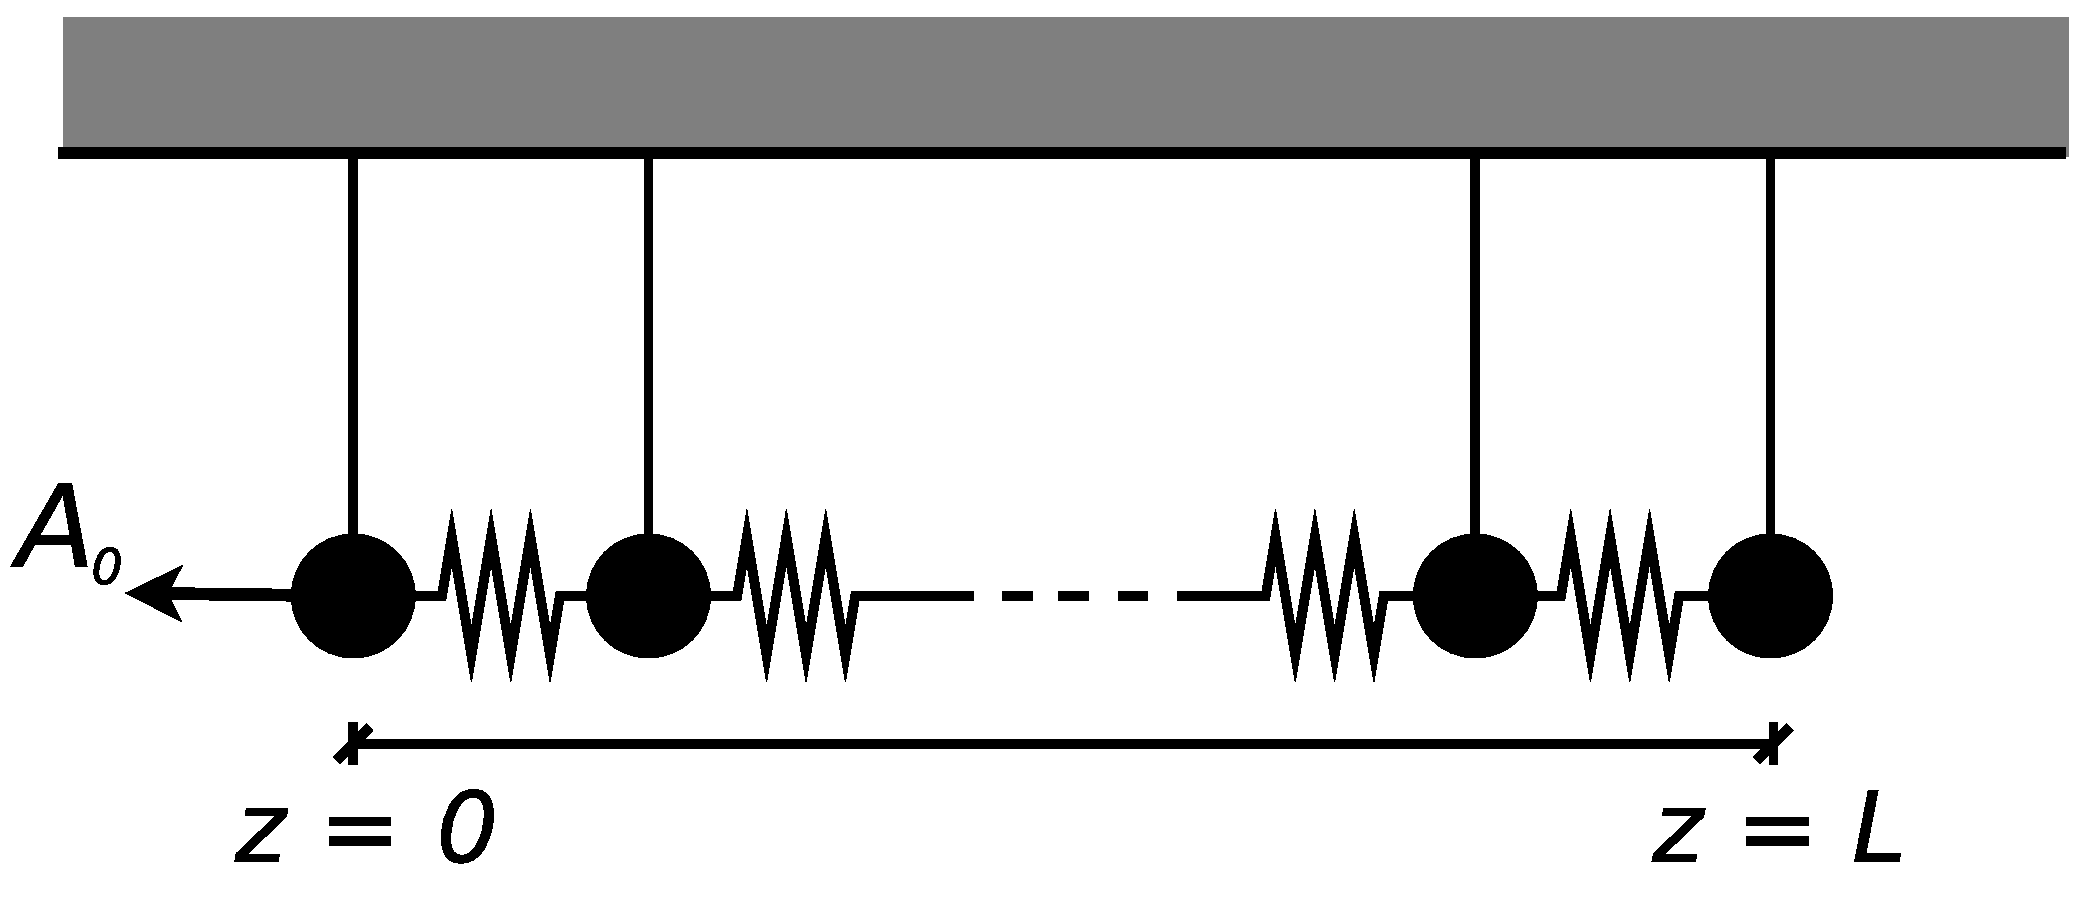
\includegraphics[width=\textwidth]{ej1-15}
\end{minipage}



\item
\begin{minipage}[t][4cm]{0.35\textwidth}
Considere un sistema de péndulos acoplados con un cambio brusco en $\omega_{0}^{2}$ en $z=L$, según se esquematiza en la figura.
Halle el movimiento estacionario del sistema y discuta las hipótesis que hace.
\end{minipage}
\begin{minipage}[c][1cm][t]{0.6\textwidth}
  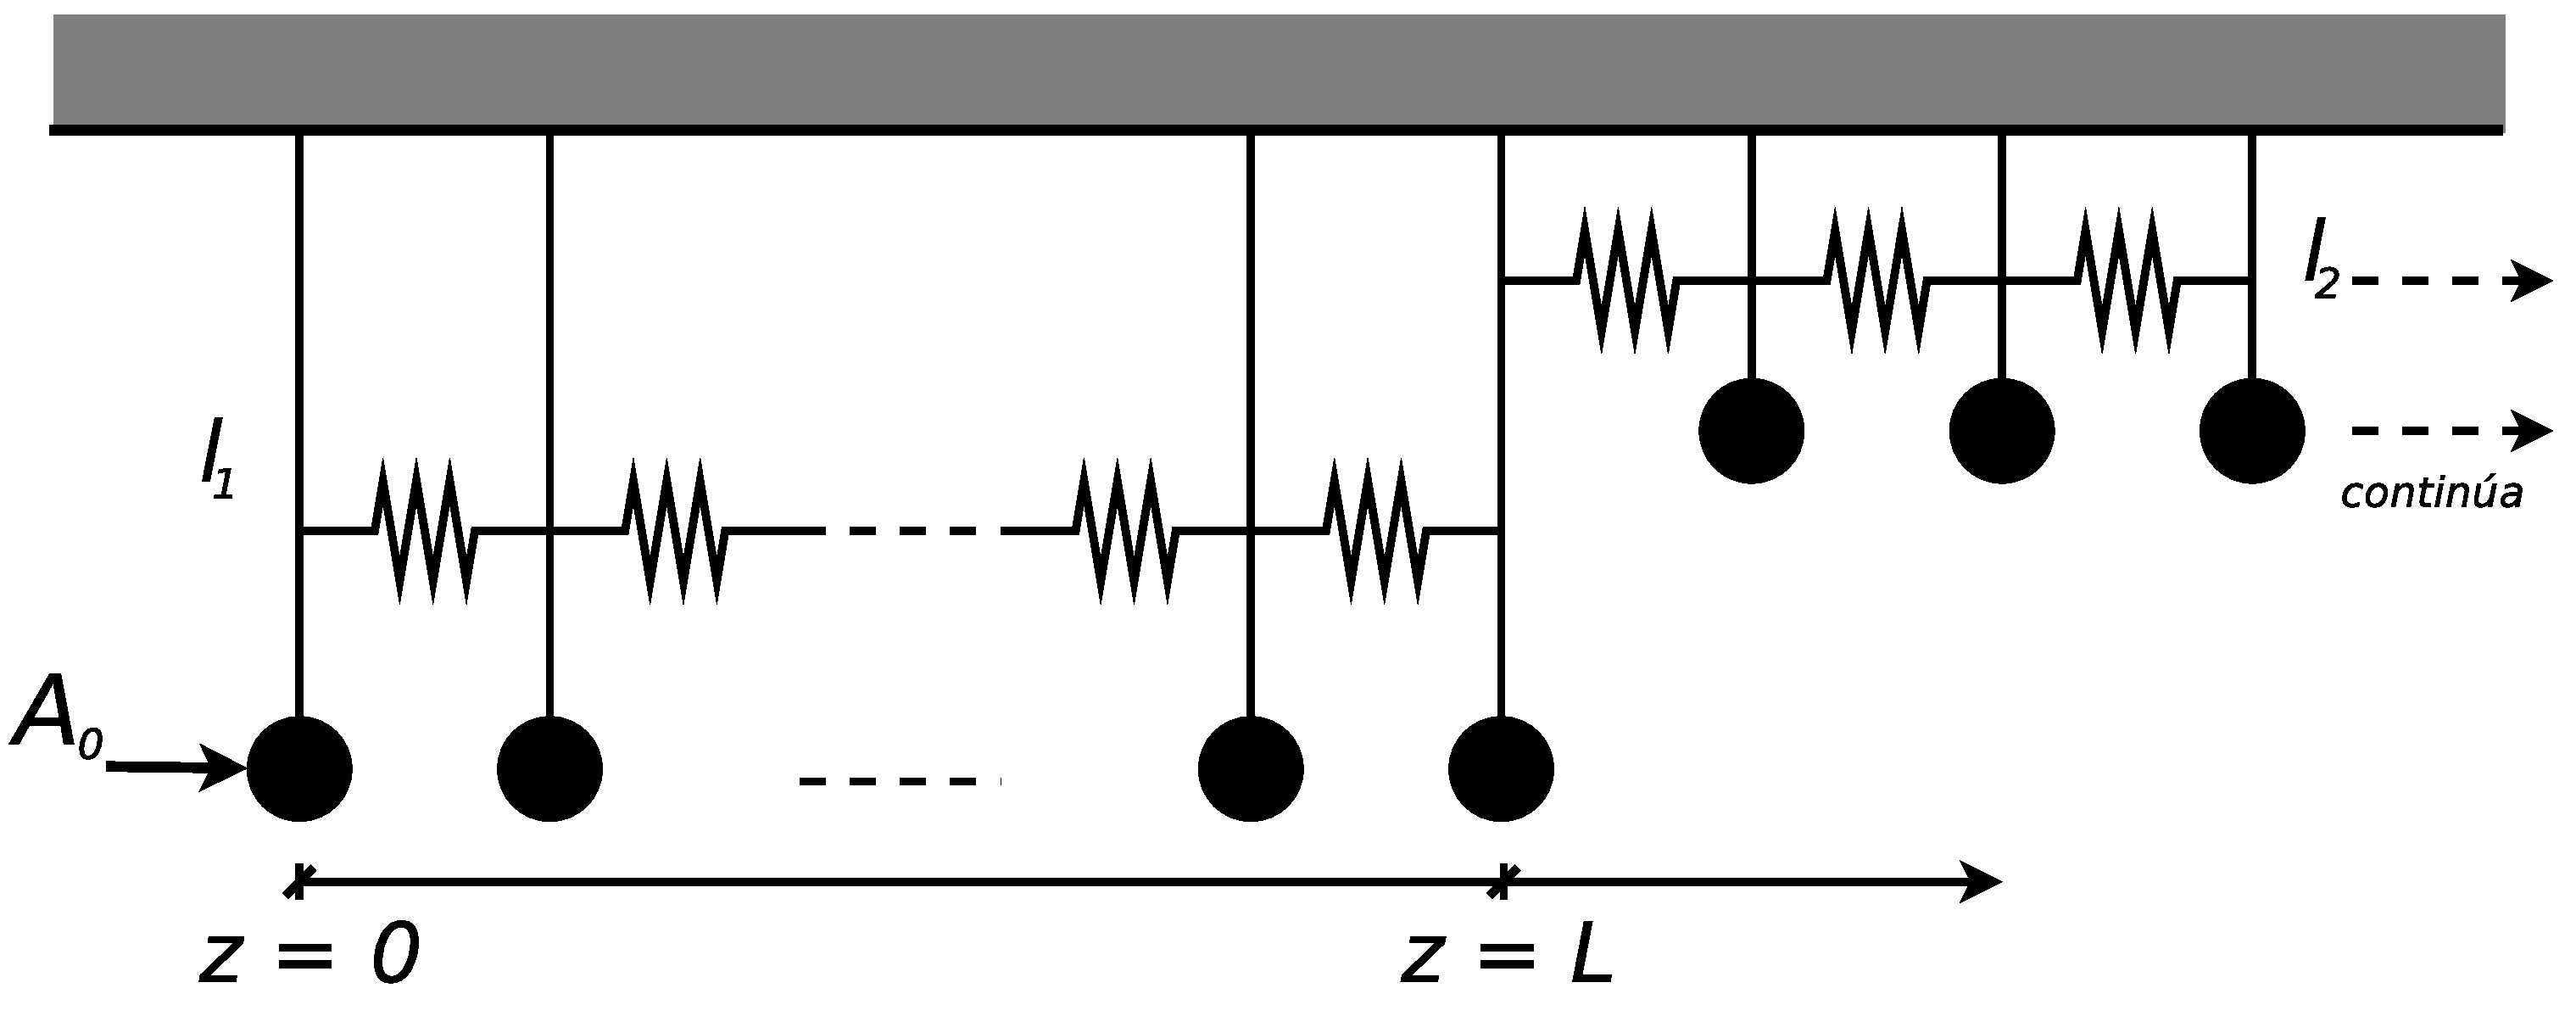
\includegraphics[width=\textwidth]{ej1-16}
\end{minipage}



\item
\begin{minipage}[t][3.5cm]{0.45\textwidth}
Para el sistema esquematizado en la figura, calcule $\Psi_{n}(t)$, si $\Omega<\omega_\textrm{mín}$.
\end{minipage}
\begin{minipage}[c][2cm][t]{0.5\textwidth}
  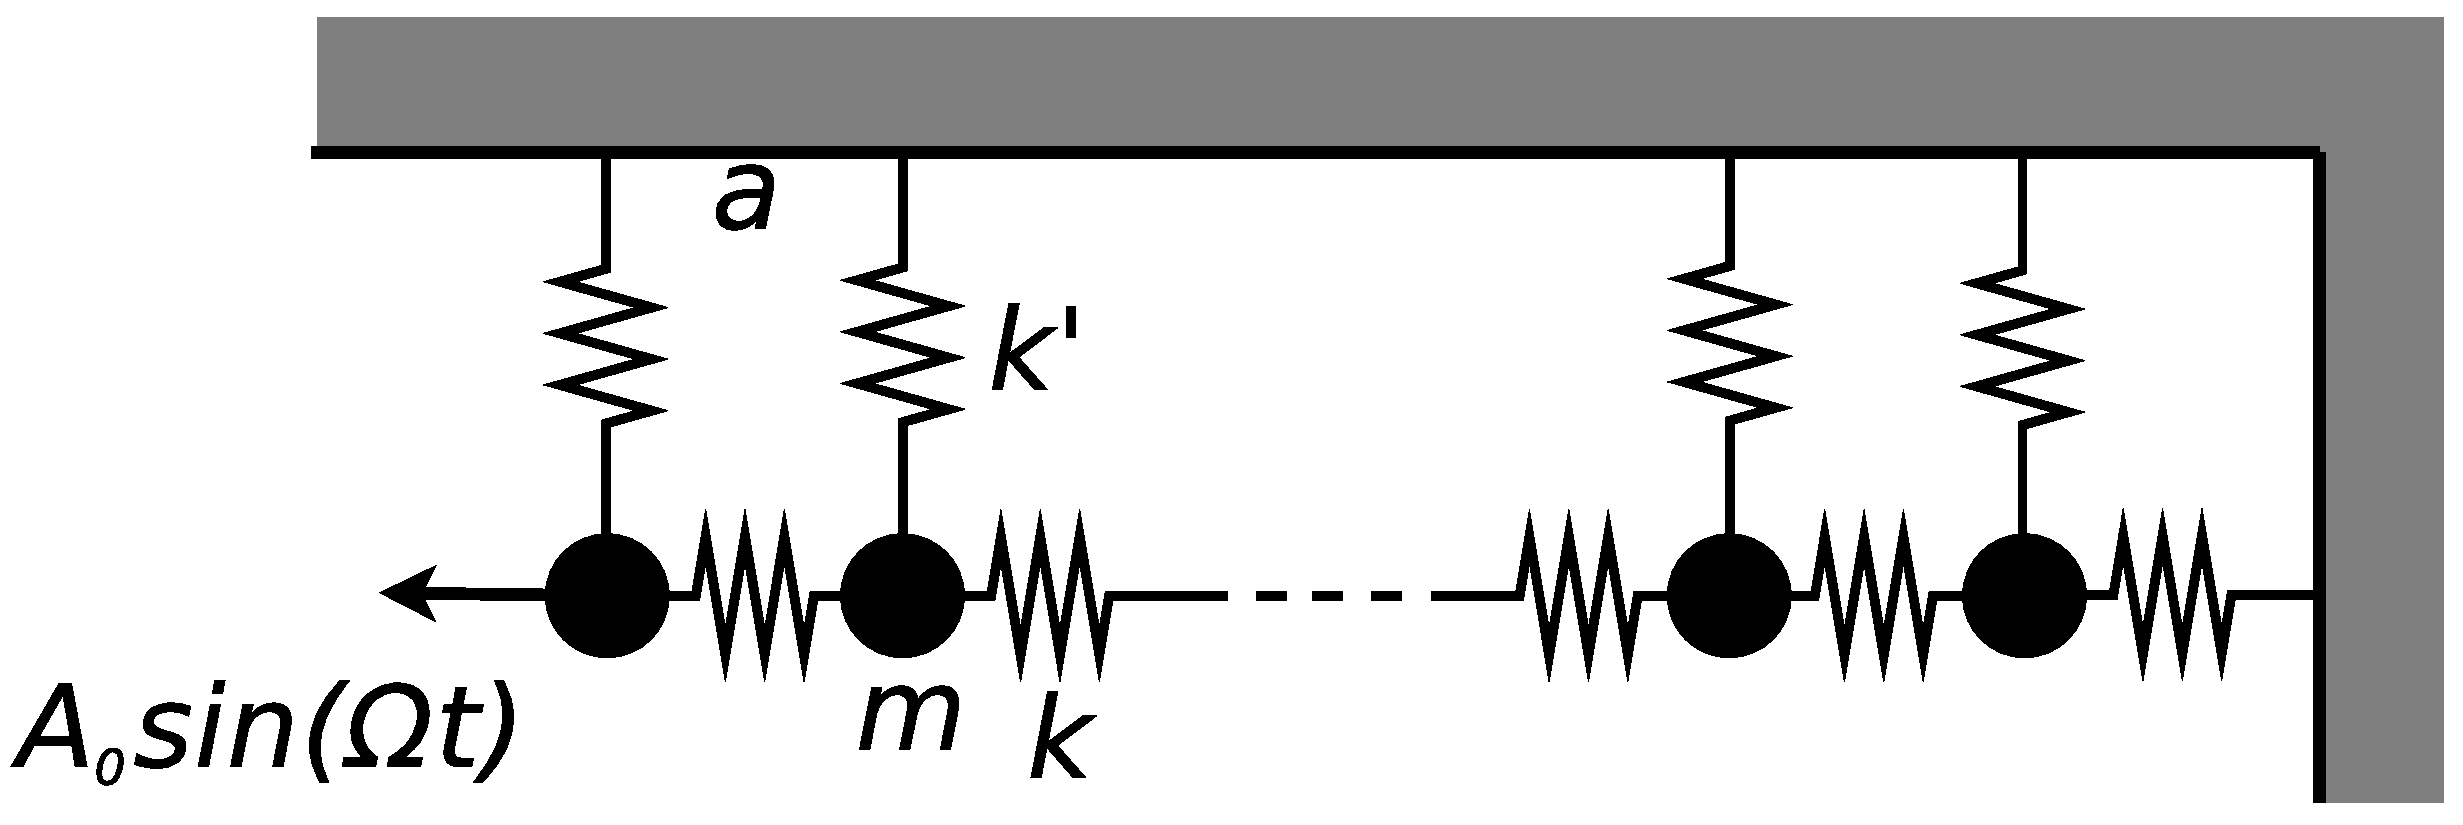
\includegraphics[width=\textwidth]{ej1-17}
\end{minipage}




\end{enumerate}

\end{document}
